\begin{enumerate}
	\item On complète le tableau par différences : lacs $= 500 - 300 = 200$ ;
	lacs satisfaisants $= 200 - 80 = 120$ ; rivières satisfaisantes $= 280 - 120 = 160$ ;
	rivières insatisfaisantes $= 300 - 160 = 140$ ; insatisfaisants $= 500 - 280 = 220$.

	\begin{center}
		\begin{tblr}{hlines, vlines,colspec={X[l,5cm]X[c,2cm]X[c,2cm]X[c,2cm]}}
			& Rivière & Lac & Total \\
			Qualité satisfaisante & \textbf{160} & \textbf{120} & 280 \\
			Qualité insatisfaisante & \textbf{140} & 80 & \textbf{220} \\
			Total & 300 & \textbf{200} & 500 \\
		\end{tblr}
	\end{center}

	\item Le choix se fait au hasard : on est en situation d'équiprobabilité.
	\begin{enumerate}
		\item $P(R) = \dfrac{300}{500} = \dfrac{3}{5}$.
		
		La probabilité que l'échantillon provienne d'une rivière est de $\frac{3}{5}$.

		\item $\overline{S}$ : \og l'échantillon choisi est classé de qualité insatisfaisante \fg.
		\[P\left(\overline{S}\right) = \dfrac{220}{500} = \dfrac{10 \times 2 \times 11}{10 \times 2 \times 25} = \dfrac{11}{25}.\]

		\item $S \cap \overline{R}$ est l'évènement \og l'échantillon est de qualité satisfaisante
		et provient d'un lac \fg.
		\[P\left(S \cap \overline{R}\right) = \dfrac{120}{500} = \dfrac{10 \times 2 \times 6}{10 \times 2 \times 25} = \dfrac{6}{25}.\]
		La probabilité que l'échantillon choisi provienne d'un lac et soit de qualité
		satisfaisante est égale à $\dfrac{6}{25}$.
	\end{enumerate}

	\item
	\begin{enumerate}
		\item $x = P_R\left(\overline{S}\right)$ est la probabilité que l'échantillon soit de qualité insatisfaisante
		sachant qu'il provient d'une rivière.

		\item Parmi les 300 échantillons provenant d'une rivière, 140 sont de qualité insatisfaisante :
		\[x = P_R\left(\overline{S}\right) = \dfrac{140}{300} = \dfrac{10 \times 2 \times 7}{10 \times 2 \times 15} = \dfrac{7}{15}.\]

		\item $P\left(\overline{R}\right) = 1 - \dfrac{3}{5} = \dfrac{2}{5}$ ; $P_R(S) = 1 - \dfrac{7}{15} = \dfrac{8}{15}$ ;
		$P_{\overline{R}}(S) = \dfrac{120}{200} = \dfrac{3}{5}$ et
		$P_{\overline{R}}\left(\overline{S}\right) = \dfrac{80}{200} = \dfrac{2}{5}$.

		\begin{center}
			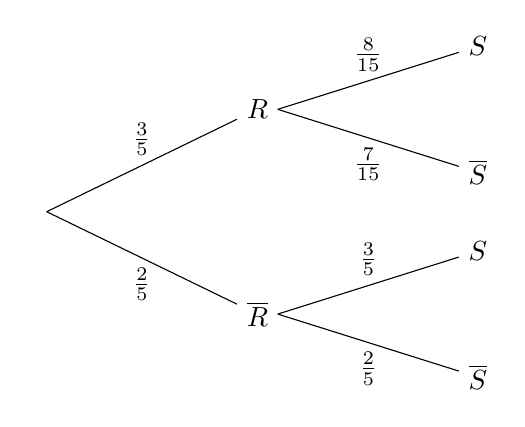
\begin{tikzpicture}[x=2.8cm, y=1cm]
				
				\node (root) at (0,0) {};
				\node (R) at (1,1.3) {$R$};
				\node (Rb) at (1,-1.3) {$\overline{R}$};
				\node (S1) at (2,2.1) {$S$};
				\node (S1b) at (2,0.5) {$\overline{S}$};
				\node (S2) at (2,-0.5) {$S$};
				\node (S2b) at (2,-2.1) {$\overline{S}$};
				
				\draw (root.east) -- (R) node[pos=0.5,above] {$\frac{3}{5}$};
				\draw (root.east) -- (Rb) node[pos=0.5,below] {$\frac{2}{5}$};
				
				\draw (R.east) -- (S1) node[pos=0.5,above] {$\frac{8}{15}$};
				\draw (R.east) -- (S1b) node[pos=0.5,below] {$\frac{7}{15}$};
				\draw (Rb.east) -- (S2) node[pos=0.5,above] {$\frac{3}{5}$};
				\draw (Rb.east) -- (S2b) node[pos=0.5,below] {$\frac{2}{5}$};
			\end{tikzpicture}
		\end{center}
	\end{enumerate}

	\item Les évènements $R$ et $\overline{S}$ sont indépendants si et seulement si
	$P\left(R \cap \overline{S}\right) = P(R) \times P\left(\overline{S}\right)$.

	D'une part $P\left(R \cap \overline{S}\right) = \dfrac{140}{500} = \dfrac{7}{25} = \dfrac{35}{125}$ ;
	d'autre part $P(R) \times P\left(\overline{S}\right) = \dfrac{3}{5} \times \dfrac{11}{25} = \dfrac{33}{125}$.

	Comme $\dfrac{35}{125} \neq \dfrac{33}{125}$, l'égalité n'est pas vérifiée.

	Les évènements \og l'échantillon provient d'une rivière \fg{} et \og l'échantillon est de qualité
	insatisfaisante \fg{} ne sont \textbf{pas indépendants}.
\end{enumerate}
